\documentclass[11pt,t]{beamer}
% xcolor and define colors -------------------------
\usepackage{xcolor}

% https://www.viget.com/articles/color-contrast/
\definecolor{purple}{HTML}{695693}
\definecolor{navy}{HTML}{567293}
\definecolor{ruby}{HTML}{9a2515}
\definecolor{alice}{HTML}{107895}
\definecolor{daisy}{HTML}{EBC944}
\definecolor{coral}{HTML}{F26D21}
\definecolor{kelly}{HTML}{829356}
\definecolor{cranberry}{HTML}{E64173}
\definecolor{jet}{HTML}{131516}
\definecolor{asher}{HTML}{555F61}
\definecolor{slate}{HTML}{314F4F}

% Main theme colors
\definecolor{accent}{HTML}{107895}
\definecolor{accent2}{HTML}{9a2515}

\newcommand\navy[1]{{\color{navy}#1}}
\newcommand\purple[1]{{\color{purple}#1}}
\newcommand\kelly[1]{{\color{kelly}#1}}
\newcommand\ruby[1]{{\color{ruby}#1}}
\newcommand\alice[1]{{\color{alice}#1}}
\newcommand\daisy[1]{{\color{daisy}#1}}
\newcommand\coral[1]{{\color{coral}#1}}
\newcommand\cranberry[1]{{\color{cranberry}#1}}
\newcommand\slate[1]{{\color{slate}#1}}
\newcommand\jet[1]{{\color{jet}#1}}
\newcommand\asher[1]{{\color{asher}#1}}

\newcommand\bgNavy[1]{{\colorbox{navy!80!white}{\textcolor{white}{#1}}}}
\newcommand\bgPurple[1]{{\colorbox{purple!80!white}{\textcolor{white}{#1}}}}
\newcommand\bgKelly[1]{{\colorbox{kelly!80!white}{\textcolor{white}{#1}}}}
\newcommand\bgRuby[1]{{\colorbox{ruby!80!white}{\textcolor{white}{#1}}}}
\newcommand\bgAlice[1]{{\colorbox{alice!80!white}{\textcolor{white}{#1}}}}
\newcommand\bgDaisy[1]{{\colorbox{daisy!80!white}{\textcolor{white}{#1}}}}
\newcommand\bgCoral[1]{{\colorbox{coral!80!white}{\textcolor{white}{#1}}}}
\newcommand\bgCranberry[1]{{\colorbox{cranberry!80!white}{\textcolor{white}{#1}}}}


% Beamer Options -------------------------------------

% Background
\setbeamercolor{background canvas}{bg = white}

% Change text margins
\setbeamersize{text margin left = 15pt, text margin right = 15pt} 

% \alert
\setbeamercolor{alerted text}{fg = accent2}

% Frame title
\setbeamercolor{frametitle}{bg = white, fg = jet}
\setbeamercolor{framesubtitle}{bg = white, fg = accent}
\setbeamerfont{framesubtitle}{size = \small, shape = \itshape}

% Block
\setbeamercolor{block title}{fg = white, bg = accent2}
\setbeamercolor{block body}{fg = jet, bg = jet!10!white}

% Title page
\setbeamercolor{title}{fg = jet}
\setbeamercolor{subtitle}{fg = accent}

%% Custom \maketitle and \titlepage
\setbeamertemplate{title page}
{
    %\begin{centering}
        \vspace{20mm}
        {\Large \usebeamerfont{title}\usebeamercolor[fg]{title}\inserttitle}\\ \vskip0.25em%
        \ifx\insertsubtitle\@empty%
        \else%
          {\usebeamerfont{subtitle}\usebeamercolor[fg]{subtitle}\insertsubtitle\par}%
        \fi% 
        {\vspace{10mm}\insertauthor}\\
        {\color{asher}\small{\insertdate}}\\
    %\end{centering}
}

% Table of Contents
\setbeamercolor{section in toc}{fg = accent!70!jet}
\setbeamercolor{subsection in toc}{fg = jet}

% Button 
\setbeamercolor{button}{bg = accent}

% Remove navigation symbols
\setbeamertemplate{navigation symbols}{}

% Optional: page numbers at bottom
\addtobeamertemplate{navigation symbols}{}{%
    \usebeamerfont{footline}%
    \hspace{1em}%
    \alice{\insertframenumber/\inserttotalframenumber}
    \vspace*{1.5mm}
}


% Table and Figure captions
\setbeamercolor{caption}{fg=jet!70!white}
\setbeamercolor{caption name}{fg=jet}
\setbeamerfont{caption name}{shape = \itshape}

% Bullet points

%% Fix left-margins
\settowidth{\leftmargini}{\usebeamertemplate{itemize item}}
\addtolength{\leftmargini}{\labelsep}

%% enumerate item color
\setbeamercolor{enumerate item}{fg = accent}
\setbeamerfont{enumerate item}{size = \small}
\setbeamertemplate{enumerate item}{\insertenumlabel.}

%% enumerate subitem color
\setbeamercolor{enumerate subitem}{fg = accent!60!white}
\setbeamerfont{enumerate subitem}{size = \small}
\setbeamertemplate{enumerate subitem}{\insertenumlabel.}

%% itemize
\setbeamercolor{itemize item}{fg = accent!70!white}
\setbeamerfont{itemize item}{size = \small}
\setbeamertemplate{itemize item}[circle]

%% right arrow for subitems
\setbeamercolor{itemize subitem}{fg = accent!60!white}
\setbeamerfont{itemize subitem}{size = \small}
\setbeamertemplate{itemize subitem}{$\rightarrow$}

\setbeamertemplate{itemize subsubitem}[square]
\setbeamercolor{itemize subsubitem}{fg = jet}
\setbeamerfont{itemize subsubitem}{size = \small}

% References

%% Bibliography Font, roughly matching aea
\setbeamerfont{bibliography item}{size = \footnotesize}
\setbeamerfont{bibliography entry author}{size = \footnotesize, series = \bfseries}
\setbeamerfont{bibliography entry title}{size = \footnotesize}
\setbeamerfont{bibliography entry location}{size = \footnotesize, shape = \itshape}
\setbeamerfont{bibliography entry note}{size = \footnotesize}

\setbeamercolor{bibliography item}{fg = jet}
\setbeamercolor{bibliography entry author}{fg = accent!60!jet}
\setbeamercolor{bibliography entry title}{fg = jet}
\setbeamercolor{bibliography entry location}{fg = jet}
\setbeamercolor{bibliography entry note}{fg = jet}

%% Remove bibliography symbol in slides
\setbeamertemplate{bibliography item}{}





% Links ----------------------------------------------

\usepackage{hyperref}
\hypersetup{
  colorlinks = true,
  linkcolor = accent2,
  filecolor = accent2,
  urlcolor = accent2,
  citecolor = accent2,
}


% Line spacing --------------------------------------
\usepackage{setspace}
% \setdisplayskipstretch{2}
\setstretch{1.3}


% \begin{columns} -----------------------------------
\usepackage{multicol}


% Fonts ---------------------------------------------
% Beamer Option to use custom fonts
\usefonttheme{professionalfonts}

% \usepackage[utopia, smallerops, varg]{newtxmath}
% \usepackage{utopia}
\usepackage[sfdefault,light]{roboto}

% Small adjustments to text kerning
\usepackage{microtype}



% Remove annoying over-full box warnings -----------
\vfuzz2pt 
\hfuzz2pt


% Table of Contents with Sections
\setbeamerfont{myTOC}{series=\bfseries, size=\Large}
\AtBeginSection[]{
        \frame{
            \frametitle{Roadmap}
            \tableofcontents[current]   
        }
    }


% References ----------------------------------------
\usepackage[
    citestyle= authoryear,
    style = authoryear,
    natbib = true, 
    backend = biber
]{biblatex}

% Smaller font-size for references
\renewcommand*{\bibfont}{\small}

% Remove "In:"
\renewbibmacro{in:}{}

% Color citations for slides
\newenvironment{citecolor}
    {\footnotesize\begin{color}{accent2}}
    {\end{color}}

\newcommand{\citetcolor}[1]{{\footnotesize\textcolor{gray}{\citet{#1}}}}
\newcommand{\citepcolor}[1]{{\footnotesize\textcolor{gray}{\citep{#1}}}}

% Tables -------------------------------------------
% Tables too big
% \begin{adjustbox}{width = 1.2\textwidth, center}
\usepackage{adjustbox}
\usepackage{array}
\usepackage{threeparttable, booktabs, adjustbox}
    
% Fix \input with tables
% \input fails when \\ is at end of external .tex file

\makeatletter
\let\input\@@input
\makeatother

% Tables too narrow
% \begin{tabularx}{\linewidth}{cols}
% col-types: X - center, L - left, R -right
% Relative scale: >{\hsize=.8\hsize}X/L/R
\usepackage{tabularx}
\newcolumntype{L}{>{\raggedright\arraybackslash}X}
\newcolumntype{R}{>{\raggedleft\arraybackslash}X}
\newcolumntype{C}{>{\centering\arraybackslash}X}

% Figures

% \imageframe{img_name} -----------------------------
% from https://github.com/mattjetwell/cousteau
\newcommand{\imageframe}[1]{%
    \begin{frame}[plain]
        \begin{tikzpicture}[remember picture, overlay]
            \node[at = (current page.center), xshift = 0cm] (cover) {%
                \includegraphics[keepaspectratio, width=\paperwidth, height=\paperheight]{#1}
            };
        \end{tikzpicture}
    \end{frame}%
}

% subfigures
\usepackage{subfigure}

% Strikeout text
\usepackage{cancel}

% Highlight slide -----------------------------------
% \begin{transitionframe} Text \end{transitionframe}
% from paulgp's beamer tips
\newenvironment{transitionframe}{
    \setbeamercolor{background canvas}{bg=accent!60!black}
    \begin{frame}\color{accent!10!white}\LARGE\centering
}{
    \end{frame}
}


% Table Highlighting --------------------------------
% Create top-left and bottom-right markets in tabular cells with a unique matching id and these commands will outline those cells
\usepackage[beamer,customcolors]{hf-tikz}
\usetikzlibrary{calc,fit,shapes.misc,backgrounds}
\usepackage{pgfplots}
\pgfplotsset{compat = newest}
\usetikzlibrary{positioning, arrows.meta}
\usepgfplotslibrary{fillbetween}

% halo around text
%https://tex.stackexchange.com/questions/18472/tikz-halo-around-text
\usepackage[outline]{contour} 
\contourlength{1.2pt}
\tikzset{
  contour text/.style={node contents={\contour{white}{#1}}},
  halo text node/.style={circle, draw, pattern=north east lines}
}


\def\arraystretch{0.75}

% To set the hypothesis highlighting boxes red.
\newcommand\marktopleft[1]{%
    \tikz[overlay,remember picture] 
        \node (marker-#1-a) at (0,1.5ex) {};%
}
\newcommand\markbottomright[1]{%
    \tikz[overlay,remember picture] 
        \node (marker-#1-b) at (0,0) {};%
    \tikz[accent!80!jet, ultra thick, overlay, remember picture, inner sep=4pt]
        \node[draw, rectangle, fit=(marker-#1-a.center) (marker-#1-b.center)] {};%
}


\author{Michael Karas}
\title{Lecture 13 - Oligopoly}
\subtitle{ECON 3070 - Intermediate Microeconomic Theory}
\date{March XX, 2025}

\begin{document}

\begin{frame}
  \titlepage
\end{frame}

\begin{frame}{Overview}
  So far we've discussed markets with either one firm or with a large number of firms.

  \begin{itemize}
    \item In this chapter, we will discuss markets with a small number of firms.
    
    \item We will look at a couple of different models of competition with two firms and discuss the resulting equilibria in each.
  \end{itemize}
\end{frame}

\begin{frame}{Market Structure}
  Below is an illustration of different market structures:

  \begin{figure}
    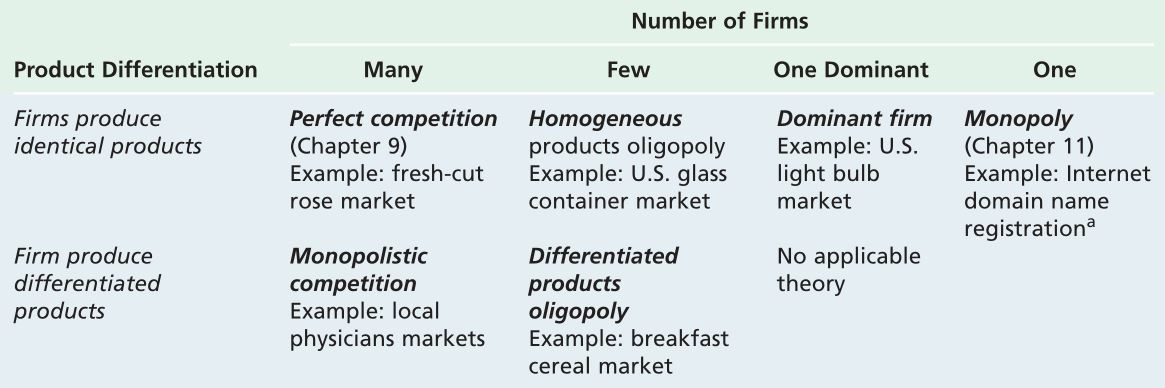
\includegraphics[width=300px]{figures/table13_1.jpg}
  \end{figure}
\end{frame}

\begin{frame}{Market Structure}
  Aside from the two that we've discussed in depth, there are four more that we will talk about:

  \bigskip
  \alice{1.} A \textbf{homogeneous products oligopoly market} is one in which there are few sellers, who all sell a similar product.
  \begin{itemize}
    \item An example is the U.S. glass container industry. Three firms account for 82\% of sales.
    \item In the market for titanium dioxide, several large firms sell almost the exact same product.
  \end{itemize}
\end{frame}

\begin{frame}{Market Structure}
  \alice{2.} In a \textbf{dominant firm market}, one large firm possesses a large share of the market but competes against many small firms.

  \begin{itemize}
    \item An example is the U.S market for light-bulbs.
    \item Many small firms compete, but GE alone counts for 50\% of sales.
  \end{itemize}
\end{frame}

\begin{frame}{Market Structure}
  \alice{3.} In \textbf{differentiated products oligopoly markets}, a small number of firms sell products that are substitutes, but differ in some way.

  \begin{itemize}
    \item Coke and Pepsi are a good example. These two firms dominate the market, but face competition from numerous smaller companies.
    
    \item In the U.S. breakfast cereal market, Kellog, General Mills, Post and Quaker Oats sell more than 85\% of all cereal.
    
    \item In Japan, Asahi, Kirin, Sapporo, and Suntory account for nearly 100\% of Japanese beer sales.
  \end{itemize}
\end{frame}

\begin{frame}{Market Structure}
  \alice{4.} Finally, \textbf{monopolistic competition} refers to a market in which many small firms produce differentiated products.

  \begin{itemize}
    \item Examples include dry cleaners, physicians, and restaurants.
  \end{itemize}
\end{frame}

\begin{frame}{Market Structure}
  Economists use various metrics to describe market structure. The \textbf{four-firm concentration ratio (4CR)} calculates the share of industry sales accounted for by the four largeset firms.

  \begin{itemize}
    \item For example, if the four largest firms have 3\%, 2\%, 2\% and 1\% of sales, then the market would have a 4CR of 8.
  \end{itemize}

  \smallskip
  Another metric is the HHI, which is the sum of square market shares for all firms.

  \begin{itemize}
    \item If one firm has all of the market share, then $HHI = 100^2 = 10,000$. This is the maximum possible value.
    
    \item On the other hand, if 100 identical firms each have 1\% of market share, $HHI = 100 * (1^2) = 100$. 
  \end{itemize}
\end{frame}

\begin{frame}{Cournot Oligopoly Model}
  An important feature of oligopoly models is competitive interdependence.

  \begin{itemize}
    \item The decisions if every firm significantly impact the profits of competitors.
  \end{itemize}

  \bigskip
  One model of oligopoly is the \textbf{Cournot model}.

  \begin{itemize}
    \item We will consider two firms in the market, but it can be extended.
  \end{itemize}
\end{frame}

\begin{frame}{Cournot Oligopoly Model}
  Firms choose output quantity simultaneously and noncooperatively (without colluding). Once quantities are chosen, price instantly adjusts.

  \begin{itemize}
    \item Firm's output choice depends on market price, and market price depends on both firms' output levels.

    \item Firm's don't know competitor's output choice, so they make their choice based on expectation.
  
    \item In other words, firm A makes output choice based on what it expects firm B to produce, and vice versa.
  \end{itemize}
\end{frame}

\begin{frame}{Cournot Oligopoly Model}
  A firm's \textbf{residual demand curve} is the demand curve that the firm faces, given its competitor's decision.

  \bigskip 
  For example, suppose firms A and B face the demand curve $P=100-Q$, where $Q = Q_1 + Q_2$.
  \begin{itemize}
    \item If firm B decides to produce 50 units, for example, then firm A faces the residual demand curve $P = 100 - Q_1 - 50$ or $P = 50 - Q_1$.
    \item Likewise, if firm B decides to produce 20 units, then firm A faces the residual demand curve $P = 80 - Q_1$.
  \end{itemize}
\end{frame}

\begin{frame}{Cournot Oligopoly Model}
  \begin{figure}
    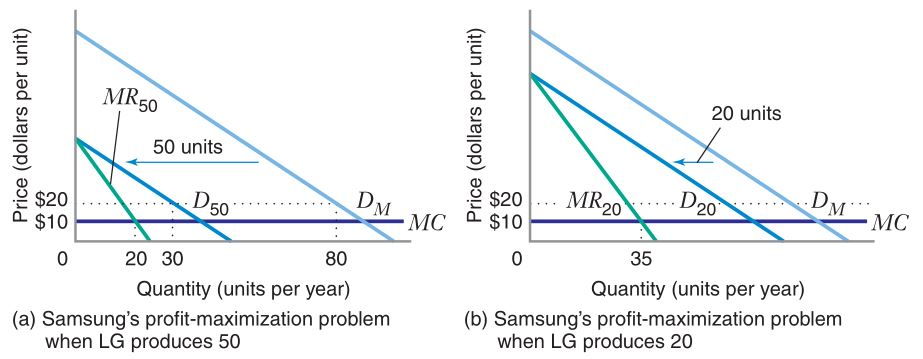
\includegraphics[width=300px]{figures/fig13_1.jpg}
  \end{figure}
\end{frame}

\begin{frame}{Cournot Oligopoly Model}
  Each firm acts as a monopolist relative to its residual demand curve.

  \begin{itemize}
    \item In other words, it sets $MR(Q_i) = MC(Q_i)$, where $MR$ is determined from their residual demand curve
  \end{itemize}
  
  \bigskip\pause
  The resulting optimal quantity will depend on the other firm's decision.

  \begin{itemize}
    \item For firm A, for example, we will find $Q_A^*(Q_B)$
  \end{itemize}

  \bigskip
  These functions for the optimal quantity are the firm's \textbf{best response functions}, or \textbf{reaction functions}
  \begin{itemize}
    \item They indicate the \textit{best response} of one firm to another firm's level of output.
  \end{itemize}
\end{frame}

\begin{frame}{Cournot Oligopoly Model}
  The \textbf{Cournot Equilibrium} is the point where the two curves intersect:
  \begin{itemize}
    \item At this intersection, neither firm has an incentive to change their quantity.
    \item That's because their quantity is the \textit{best response} to the other firm's output choice.
  \end{itemize}
\end{frame}

\begin{frame}{Cournot Oligopoly Model}
  Below are the best response functions of two firms in a duopoly. The intersection of their curves is the Cournot Equilibrium
  \begin{figure}
    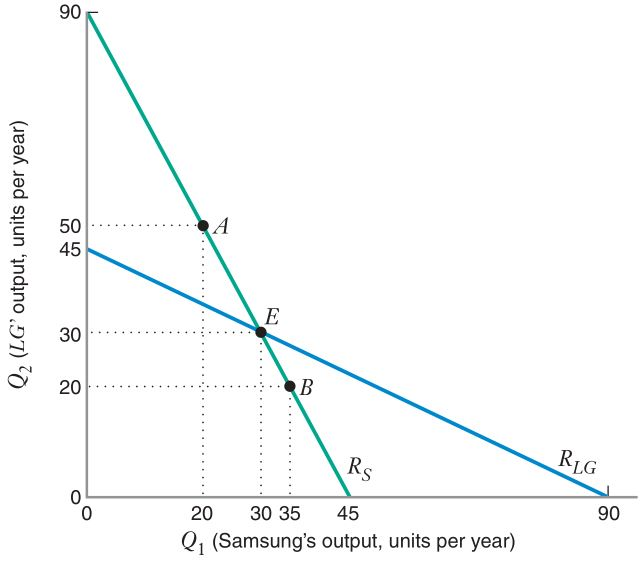
\includegraphics[width=180px]{figures/fig13_2.jpg}
  \end{figure}
\end{frame}

\begin{frame}{\bgCranberry{Try It Yourself}}
  In the Cournot model, the firm chooses

  \begin{enumerate}[A)]
    \item its optimal price, holding the price of its competitors constant.
    \item its best response to the price changes of the competitor firm.
    \item its optimal level of output, holding the output of the other firm constant.
    \item the level of output that would optimize profits for all firms.
  \end{enumerate}
\end{frame}

\begin{frame}{Cournot Oligopoly Model}
  Example: Suppose that market demand is given by $P=100-Q_1-Q_2$, where $Q_1$ and $Q_2$ are the amount of output produced by firms 1 and 2, respectively. Marginal cost for each firm is \$10.

  \medskip
  Firm 1's marginal revenue function can be found by taking the derivative of $P*Q$:
  $$
    MR(Q_1)=\frac{\partial (100Q_1-Q_1^2-Q_1Q_2)}{\partial Q_1} = 100 - 2Q_1 - Q_2
  $$
  Likewise for firm 2:
  $$
    MR(Q_2)=\frac{\partial (100Q_1-Q_1Q_2-Q_2^2)}{\partial Q_1} = 100 - Q_1 - 2Q_2
  $$
\end{frame}

\begin{frame}{Cournot Oligopoly Model}
  Firm 1's best response function is found by setting $MR(Q_1) = MC(Q_1)$:
  $$
    100 - 2Q_1 - Q_2 = 10 \implies Q_1^* = 45 - \frac{1}{2} Q_2
  $$
  Likewise for firm 2:
  $$
    100 - Q_1 - 2Q_2 = 10 \implies Q_2^* = 45 - \frac{1}{2} Q_1
  $$
\end{frame}

\begin{frame}{Cournot Oligopoly Model}
  To find the Cournot equilibrium, we simply solve the system of two equations. Let's plug firm 2's BR function in to firm 1's BR function.
  $$
    Q_1 = 45 - \frac{1}{2} (45 - \frac{1}{2} Q_1) = 22.5 + \frac{1}{4} Q_1
  $$
  Solving for $Q_1^*$:
  $$
    \frac{3}{4}Q_1 = 22.5 \implies Q_1 = 30 \implies Q_2 = 45 - \frac{1}{2} * 30 = 30
  $$
  
  Finally, plugging this into the demand curve gives us the price $P^* = 100 - Q_1 - Q_2 = 100 - 30 - 30 = 40$.
\end{frame}

\begin{frame}{Cournot Oligopoly Model}
  Note that the equilibrium price is above marginal cost, so this does not correspond to the perfectly competitive equilibrium. However, as the number of firms increases in this model, total profit falls.

  \begin{figure}
    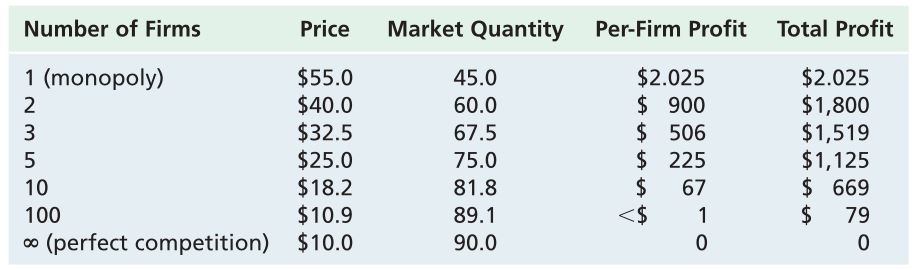
\includegraphics[width=300px]{figures/table13_4.jpg}
  \end{figure}
\end{frame}

\begin{frame}{\bgCranberry{Try It Yourself}}
  Suppose that firms A and B are Cournot duopolists in the salt industry.  The market demand curve can be specified as $P = 200 - Q_A - Q_B$.  The marginal cost to each firm is \$40. What is firm B's profit-maximizing quantity when firm A produces an arbitrary output $Q_A$?
\end{frame}

\begin{frame}{Bertrand Model of Oligopoly}
  The \textbf{Bertrand model of oligopoly} assumes that firms each select a selling price.

  \begin{itemize}
    \item Consumers know both prices, and will purchase from whomever has the lowest price.
    \item Once a firm sets their price, they are able to supply as many units as consumers want.
    \item If one firm sets their price lower than the other, they will capture all of the demand in the market.
  \end{itemize}
\end{frame}


\begin{frame}{Bertrand Model of Oligopoly}
  A \textbf{Bertrand equilibrium} occurs when each firm chooses their profit-maximizing price, given the price set by the other firm.

  \bigskip 
  Going back to our previous example, suppose two firms compete in a duopoly market. Both firms face a marginal cost of \$10.

  \begin{itemize}
    \item Suppose that both firms initially charge \$40 for a unit of the good.
    \item If firm A decides to undercut firm by by \$1, they will capture the whole market.
  \end{itemize}

\end{frame}


\begin{frame}{Bertrand Model of Oligopoly}
  But then firm B will have an incentive to lower their price.
  \begin{itemize}
    \item They would keep competing in this way until the price was equal to their marginal cost (it's turtles all the way down).
    \item Beyond that point, if they lowered their price more, profit would be negative.
  \end{itemize}

  \bigskip\pause
  The result is that both firms charge their marginal cost, and neither firm makes a profit.

  \begin{itemize}
    \item Compare this to the Cournot model, where the firms both charged a price above MC.
  \end{itemize}
\end{frame}


\begin{frame}{Comparing Bertrand and Cournot}
  Why are the results of these two oligopoly models so different?

  \begin{itemize}
    \item Cournot can be thought of as taking place over a longer time period.
    \item Firms choose their capacity and then compete as price setters.
    \item In contrast, Bertrand can be though of as short-run, where both firms have enough capacity to satisfy market demand.
  \end{itemize}
\end{frame}


\begin{frame}{Comparing Bertrand and Cournot}
  Cournot oligopolists expect competitors to adjust prices immediately to keep sales constant.

  \begin{itemize}
    \item So one firm cannot quickly undercut the other to steal their sales.
  \end{itemize}
  
  \bigskip
  In Bertrand, the opposite is true.

  \begin{itemize}
    \item Each firm knows it's competitors may undercut its price, so they behave more aggressively by keeping their price lower.
  \end{itemize}
\end{frame}

\end{document}
